\documentclass[12pt,fleqn]{article}
\setlength{\parindent}{0pt}
\usepackage{graphicx}
\usepackage{cancel}
\usepackage{listings}
\usepackage[latin5]{inputenc}
\usepackage{color}
\setlength{\parskip}{8pt}
\setlength{\parsep}{0pt}
\setlength{\headsep}{0pt}
\setlength{\topskip}{0pt}
\setlength{\topmargin}{0pt}
\setlength{\topsep}{0pt}
\setlength{\partopsep}{0pt}
\setlength{\mathindent}{0cm}
\usepackage{latexsym}
\usepackage{showkeys}
\renewcommand*\showkeyslabelformat[1]{(#1)}

\begin{document}
Ders 22

Muhendislerin Laplace Transformunu sevmesinin sebeplerinden biri
fonksiyonlarda kesintili / birdenbire ziplayan gecisleri (jump
discontinuities) durumlarinda bozulmadan isleyebiliyor olmasidir. 

Kesintili fonksiyonlardan biri birim adim fonksiyonudur. Fonksiyonun
kendisi tartisma yaratan bir fonksiyon aslinda, sifir noktasinda hangi
degere sahip oldugu hala kararlastirilamadi. Bazilari 0 diyor, bazilari 1
diyor, ben bu derste tanimsiz birakacagim. Yani

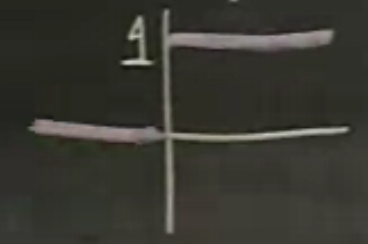
\includegraphics[height=2cm]{22_1.png}

$u(t)$ birim adim

$u(0)$ tanimsiz

Bazen sifir yerine baska bir noktada ziplama olmasini isteyebilirim. O
zaman fonksiyonu kaydirmak mumkun, mesela $a$ kadar. 

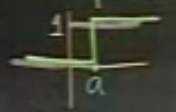
\includegraphics[height=2cm]{22_2.png}

\[ u_a(t) = u(t-a) \]

Birim Kutu

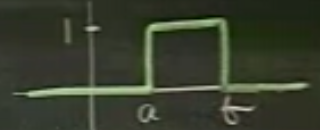
\includegraphics[height=2cm]{22_3.png}

Kutuyu birim adimlar kullanarak temsil edebilirsek iyi olur, cunku
birim adimlarin Laplace transformunu biliyoruz. 

\[ u_{ab} := u_a(t) - u_b(t) \]

\[ = u(t-a) - u(t-b) \]

Mantikli gozukuyor, $b$'ye gelene kadar birim adim gibi gidiyoruz, $b$'de
birim adimi iptal edecek sekilde birim adimi cikartiyoruz. 

Peki bu fonksiyonlar niye faydali? Diger fonksiyonlari carptiklarinda o
fonksiyonlari faydali sekillerde degistirebildikleri icin. Diyelim ki soyle
bir $f(t)$ var.

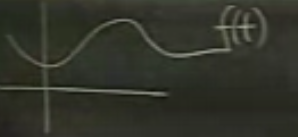
\includegraphics[height=2cm]{22_4.png}

\[ u_{ab}f(t) \]

neye benzerdi? Eger $a,b$ arasinda $u_{ab}$ 1 degerine esitse, carpim bu
aralikta $f(t)$'yi oldugu gibi alir. Diger noktalarda sifir yapar. Alttaki
sekil ortaya cikar (mavi cizgiler). 

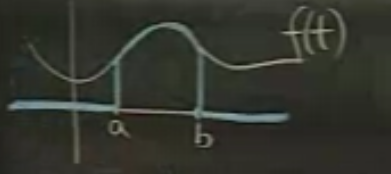
\includegraphics[height=3cm]{22_5.png}


























\end{document}
